\chapter{Estado da Arte}
% OU \chapter{Trabalhos Relacionados}
% OU \chapter{Engenharia de Software}
% OU \chapter{Tecnologias e Ferramentas Utilizadas}
\label{chap:estado-da-arte}

\section{Introdução}
\label{chap2:sec:intro}
O \hyperref[chap:estado-da-arte]{Capítulo 2} vai ser apresentado um modelo de redação de notícias, que se mostrou bastante útil neste projeto.

\section{Modelo pirâmide invertida}
\label{chap2:sec:...}
A notícia não é mais do que texto jornalístico relativo a um conteúdo factual e relata acontecimentos de interesse geral com a menor subjetividade possível.
O texto da notícia deve ser escrito com clareza, simplicidade e exatidão, assim como o bom uso do português e do cumprimento da gramática.
Uma notícia presente na \emph{Internet}, requer um tratamento diferente das demais, estas combinam texto som e imagem.\par
O modelo pirâmide invertida, tem uma função interessante no que diz respeito à redação de notícias, consiste em apresentar primeiro as informações mais importantes e na sequência da notícia apresentar as informações menos importantes. Isto permite ao leitor ter uma noção do que será apresentado ao longo da notícia, só através do primeiro parágrafo.

\vspace{0,07cm}
\begin{figure}[H]
\centering
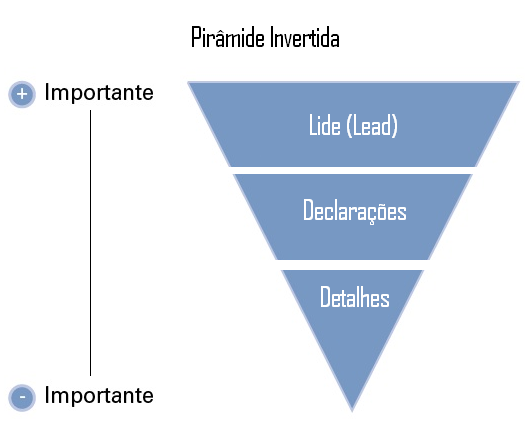
\includegraphics[scale=0.5]{relatorio-projeto/imagens/piramide_invertida.png}
\caption{Pirâmide invertida.}
\label{fig:pirâmide}
\end{figure}
 
 Na \hyperref[fig:pirâmide]{Figura 2.1} observamos que a pirâmide começa com o \emph{Lide(Lead)}, este não é mais do que a introdução da notícia. É onde se situa o leitor com os factos que aconteceram, deve conter respostas às seguintes perguntas: 'O que?', "Quando?", "Quem?", "Como?", "Onde?" e principalmente "Porque?".
 A secção \emph{Declarações} tem como objetivo desenvolver a notícia, suportando-a com informações, entrevistas ou referências.
 À medida que o notícia se desenrola os \emph{Detalhes} cada vez menos importantes por isso têm a posição mais baixa para pirâmide.
 \par
Com base neste modelo utiliza-se o primeiro parágrafo de uma notícia para ser mostrado na aplicação desenvolvida.
 
